\documentclass[12pt]{../../oss-apphys-exam}

\runningheader{
  \fontfamily{phv}\small
  \textcolor{gray}{AP PHYSICS C: ELECTRICITY AND MAGNETISM $\blacksquare$}
  \textbf{FREE-RESPONSE QUESTIONS}}{}{}


\begin{document}
\begin{center}
  {\fontfamily{phv}\Large\textbf{PHYSICS C: ELECTRICITY AND MAGNETISM\\
      SECTION II\\
      TIME -- 80 MINUTES
    }
  }
\end{center}


\vspace{2in}
\textbf{Directions:}

Section II has 4 questions and lasts 60 minutes.

You may use the available paper for scratch work and planning, but you must
write your answers in the free-response booklet. Label parts (e.g., A, B, C)
and sub-parts (e.g., i, ii, iii) as needed. Use a pencil or a pen with black or
dark blue ink to write your responses.

A calculator is allowed in this section, as well as a ruler and straightedge.
You may use a handheld four-function, scientific, or graphing calculator, or
the calculator available in this application. Reference information, including
lists of equations, can also be accessed in this application and is available
throughout the exam.

All final numerical answers should include appropriate units when applicable.
Credit for your work depends on demonstrating that you know which physical
principles to apply in a particular situation. Credit will be awarded only for
work that is clearly designated as the solution to a specific part of a
question. Credit also depends on the quality of your solutions and explanations.
Therefore, you should show your work for each part in the space provided for
that part. If you need more space, be sure to clearly indicate where you
continue your work. When constructing a graph or diagram, use only one color of
ink or pencil.

You may pace yourself as you answer the questions in this section, or you may
use these optional timing recommendations:

It is suggested that you spend about 20 minutes on each question.

You can go back and forth between questions in this section until time expires.
The clock will turn red when 5 minutes remain---\textbf{the proctor will not
  give you any time updates or warnings.}
\newpage

\begin{questions}
  \uplevel{
    \centering
    \begin{tikzpicture}[thick,transform shape]
      \fill circle (.06) node[above]{$P$};
      \fill (-1,0) circle (.06) node[above]{$e^-$};
      \draw[dashed,thick] (0,0) arc (90:0:2);
      \foreach \y in {.75,-2} \draw[line width=2.2] (0,\y)--+(4,0);
      \draw[<->] (3.5,.75)--(3.5,-2) node[midway,fill=white]{$D$};
      \draw[|<->|] (0,-2.3)--(2,-2.3) node[midway,fill=white]{$y_0$};
      \draw[<->|] (-.5,0)--(-.5,-2) node[midway,fill=white]{$y_0$};
      \draw[dashed,->] (-4.45,0)--(-.2,0);
      \begin{scope}[very thick]
        \draw (-2,.6)--(-5,.6)--(-5,-.6)--(-4.8,-.6);
        \draw (-4.6,-.6)--(-2,-.6);
        \draw (-4.7,.55)--(-4.7,.2) arc (90:-90:.2)--(-4.7,-1.1)
        to[battery,l_=$\mathcal E$] (-2.3,-1.1)--(-2.3,-.1);
        \draw (-2.3,.1)--(-2.3,.6);
      \end{scope}
    \end{tikzpicture}
  }

  \question Electrons created at the filament at the left end of the tube
  represented above are accelerated through a voltage $\mathcal E$ and exit the
  tube. The electrons then move with constant speed to the right, as shown,
  before entering a region in which there is a uniform electric field between
  two parallel plates separated by a distance $D$. The electrons enter the
  field at point $P$, which is a distance $y_0$ from the bottom plate, and are
  deflected toward that plate. Express your answers to the following in terms of
  $\mathcal E$, $D$, $y_0$, and fundamental constants.
  \begin{parts}
    \part\textbf{Derive} an algebraic expression for the speed of the electrons
    as they exit the tube.
    \vspace{\stretch{.5}}
    
    \part\textbf{Derive} an algebraic expression for the magnitude of the
    electric field required to cause the electrons to land the distance $y_0$
    from the edge of the plate.
    \vspace{\stretch1}
    
    \part\textbf{Indicate} the direction of the electric field.

    \vspace{.1in}
    \underline{\hspace{.6in}} To the left\\
    \underline{\hspace{.6in}} Toward the top of the page\\
    \underline{\hspace{.6in}} Into the page\\
    \underline{\hspace{.6in}} To the right\\
    \underline{\hspace{.6in}} Toward the bottom of the page\\
    \underline{\hspace{.6in}} Out of the page

    \vspace{.1in}\textbf{Justify} your answer.
    \vspace{\stretch1}
    
    \part\textbf{Derive} an algebraic expression for absolute value of the
    potential difference ($|\Delta V|$) between the two plates required to
    produce the electric field determined in part \textbf{B}.
    \vspace{\stretch1}
    \newpage
    
    \uplevel{
      Suppose the electric field between the plates is replaced by a magnetic
      field and the electrons are to strike the lower plate at the same
      distance $y_0$ from the edge of the plate.
    }
    \part\textbf{Derive} an algebraic expression for the magnitude of the
    magnetic field.
    \vspace{\stretch1}
    \part\textbf{Indicate} the direction of the required magnetic field.

    \vspace{.2in}
    \underline{\hspace{.6in}} To the left\\
    \underline{\hspace{.6in}} Toward the top of the page\\
    \underline{\hspace{.6in}} Into the page\\
    \underline{\hspace{.6in}} To the right\\
    \underline{\hspace{.6in}} Toward the bottom of the page\\
    \underline{\hspace{.6in}} Out of the page

    \vspace{.1in}\textbf{Justify} your answer.
    \vspace{\stretch3}
  \end{parts}
  \newpage

   % TAKEN FROM THE 2002 AP PHYSICS C E&M EXAM QUESTION #1. THE QUESTION ITSELF
  % HAS NOT CHANGED, BUT WE HAVE CHANGED THE FORMATTING TO REFLECT THE MORE
  % RECENT WAYS OF WRITING QUESTIONS.
  \uplevel{
    \centering
    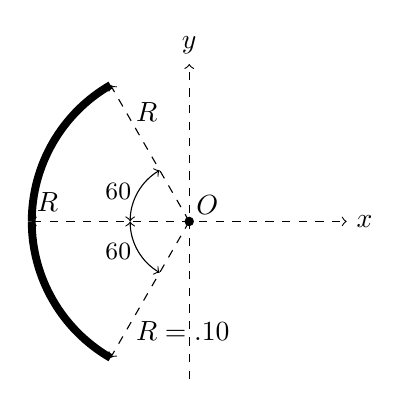
\begin{tikzpicture}
      \begin{scope}[dashed]
        \draw[<->] (-2,0)--(2,0) node[pos=.05,above]{$R$} node[right]{$x$};
        \begin{scope}[->]
          \draw (0,-2)--(0,2) node[above]{$y$};
          \draw[rotate=-60] (0,0)--(-2,0) node[pos=.8,right]{$R$};
          \draw[rotate=60] (0,0)--(-2,0) node[pos=.8,right]{$R=\SI{.10}\metre$};
        \end{scope}
      \end{scope}
      \foreach \theta in {120,240}
      \draw[<->] (-.75,0) arc (180:\theta:.75) node[midway,left=-1]{
        \small\SI{60}\degree};
      \draw[line width=1mm] (-2,0) arc (180:120:2);
      \draw[line width=1mm] (-2,0) arc (180:240:2);
      \fill circle (.06) node[above right=-1]{$O$};
    \end{tikzpicture}
  }
  \question A rod of uniform linear charge density
  $\lambda=+\SI{1.5e5}{\coulomb\per\metre}$ is bent into an arc of radius
  $R=\SI{.10}\metre$. The arc is placed with its center at the origin of the
  axes shown above.
  \begin{parts}
    \part\textbf{Calculate} the total charge on the rod.
    \vspace{\stretch1}
    
    \part\textbf{Calculate} the magnitude of the electric field at the center
    $O$ of the arc.
    \vspace{\stretch1}
    
    \part\textbf{Calculate} the electric potential at point $O$.
    \vspace{\stretch1}
    
    \uplevel{
      A proton is now placed at point $O$ and held in place. Ignore the effects
      of gravity in the rest of this problem.
    }

    \part\textbf{Calculate} the magnitude and direction of the force that must
    be applied in order to keep the proton at rest.
    \vspace{\stretch1}
    
    \part The proton is now released. \textbf{Describe} in words its motion for
    a long time after its release.
    \vspace{\stretch1}
  \end{parts}
  \newpage
  
  % TAKEN FROM THE 1999 AP PHYSICS C E&M EXAM QUESTION #3. THE QUESTION ITSELF
  % HAS NOT CHANGED, BUT WE HAVE CHANGED THE FORMATTING TO REFLECT THE MORE
  % RECENT WAYS OF WRITING QUESTIONS.
  
  \uplevel{
    \cpic{.3}{loop}
  }
  \question The non-conducting ring of radius R shown above lies in the
  $yz$-plane and carries a uniformly distributed positive charge $Q$.
  \begin{parts}
    \part\textbf{Determine} the electric potential at points along the $x$-axis
    as a function of $x$.
    \vspace{\stretch1}
    
    \part\textbf{Show} that the $x$-component of the electric field along the
    $x$-axis is given by
    \begin{displaymath}
      E_x=\frac{Qx}{4\pi\varepsilon_0(R^2+x^2)^{\frac 32}}
    \end{displaymath}
    \vspace{\stretch1}
    
    \part What are the $y$- and $z$-components of the electric field along the
    $x$-axis? \textbf{Justify} your answer.
    \vspace{\stretch1}
    \newpage
    
    \part\textbf{Determine} the value of $x$ for which $E_x$ is a maximum
    \vspace{\stretch1}
    
    \part\textbf{Determine} the maximum electric field $E_{x,\text{max}}$
    \vspace{\stretch1}
    
    \part On the axes below, \textbf{sketch} $E_x$ versus $x$ for points along
    the $x$-axis from $x=-2R$ to $x=+2R$.
    \uplevel{
      \centering
      \begin{tikzpicture}[thick]
        \draw[axes] (-8,0)--(8,0) node[right]{$x$};
        \draw[axes] (0,-2)--(0,2) node[above]{$E_x$};
        \draw (-6,.1)--(-6,-.1) node[below]{$-2R$};
        \draw (-3,.1)--(-3,-.1) node[below]{$-R$};
        \draw (3,.1)--(3,-.1) node[below]{$R$};
        \draw (6,.1)--(6,-.1) node[below]{$2R$};
      \end{tikzpicture}
    }
    \part An electron is placed at $x=R/2$ and released from rest.
    \textbf{Describe} its motion after it is released.
    \vspace{\stretch1}
  \end{parts}
  \newpage

  % TAKEN FROM THE 2000 AP PHYSICS C E&M EXAM QUESTION E&M3. THE QUESTION ITSELF
  % HAS NOT CHANGED, BUT WE HAVE CHANGED THE FORMATTING TO REFLECT THE MORE
  % RECENT WAYS OF WRITING QUESTIONS.
  \uplevel{
    \centering
    \pic{.55}{capacitor1}
  }
  \question A capacitor consists of two conducting, coaxial, cylindrical shells
  of radius $a$ and $b$, respectively, and length $L\gg b$. The space between
  the cylinders is filled with oil that has a dielectric constant $\kappa$.
  Initially both cylinders are uncharged, but then a battery is used to charge
  the capacitor, leaving a charge $+Q$ on the inner cylinder and $-Q$ on the
  outer cylinder, as shown above. Let $r$ be the radial distance from the axis
  of the capacitor.
  \begin{parts}
    \part Using Gauss's law, \textbf{determine} the electric field midway along
    the length of the cylinder for the following values of $r$, in terms of the
    given quantities and fundamental constants. Assume end effects are
    negligible.
    \begin{subparts}
      \subpart $a < r < b$
      \subpart $b < r \ll L$
    \end{subparts}
    \vspace{\stretch1}
    
    \part\textbf{Determine} the following in terms of the given quantities and
    fundamental constants.
    \begin{subparts}
      \subpart The potential difference across the capacitor
      \subpart The capacitance of this capacitor
    \end{subparts}
    \vspace{\stretch1}
    \newpage

    \uplevel{
    \centering
    \pic{.6}{ampere1}
  }
    \part Now the capacitor is discharged and the oil is drained from it. As
    shown above, a battery of emf $\mathcal{E}$ is connected to opposite ends
    of the inner cylinder and a battery of emf $3\mathcal{E}$ is connected to
    opposite ends of the outer cylinder. Each cylinder has resistance $R$.
    Assume that end effects and the contributions to the magnetic field from
    the wires are negligible. Using Ampere's law, \textbf{determine} the
    magnitude $B$ of the magnetic field midway along the length of the
    cylinders due to the current in the cylinders for the following values of
    $r$.
    \begin{subparts}
      \subpart $a < r < b$
      \subpart $b < r \ll L$
    \end{subparts}
  \end{parts}  
\end{questions}
\end{document}
